\chapter{Instalación y uso del repositorio}
\label{ap:instalacion}

Todo el código que se ha utilizado en este trabajo está disponible en un repositorio público de Git.
El objetivo de este apéndice es dar las indicaciones mínimas para que cualquier lector pueda clonar el repositorio,
instalar las dependencias y reproducir los experimentos sobre los que se construye el capítulo~\ref{cap:analisis}.

\section{Estructura del repositorio}

El repositorio se organiza con dos ramas separadas. La rama \texttt{feat/code} contiene el código fuente,
los tests unitarios y los resultados (la rama \texttt{feat/docs} contiene la memoria en \LaTeX{}, que es la que se está leyendo).
La separación entre ambas permite trabajar de forma independiente en el código y en la memoria
sin que un cambio en una parte afecte al historial de la otra.

Dentro de \texttt{feat/code}, el árbol de directorios es el siguiente.

\begin{lstlisting}[basicstyle=\small\ttfamily,frame=single,backgroundcolor=\color{gray97},numbers=none]
src/
  lfsr.py                  # LFSR generico
  berlekamp_massey.py      # algoritmo de Berlekamp-Massey
  tests_nist/              # ocho tests del estandar NIST SP 800-22
    monobit.py
    block_frequency.py
    runs.py
    binary_matrix.py
    maurer.py
    serial.py
    spectral.py
    linear_complexity.py
  generators/              # generadores basados en LFSR
    geffe.py
    shrinking.py
    self_shrinking.py
    alternating_step.py
  analysis/
    run_experiments.py     # script principal de experimentos
    plots.py               # generacion de figuras

tests/                     # tests unitarios (pytest)
results/                   # resultados generados (JSON + PNGs)
requirements.txt           # dependencias Python
\end{lstlisting}

\section{Requisitos}

El código está escrito en Python~3.10 o superior y depende de tres librerías externas.
\texttt{numpy} se usa para las operaciones sobre arrays de bits y para la FFT del test espectral,
\texttt{scipy} aporta las funciones especiales (gamma incompleta y función de error complementaria)
que necesitan varios tests estadísticos, y \texttt{matplotlib} se utiliza para generar las gráficas de complejidad lineal
y de comparación entre generadores. \texttt{pytest} se usa solo para ejecutar los tests unitarios.

Las versiones mínimas están fijadas en \texttt{requirements.txt}.

\begin{lstlisting}[basicstyle=\small\ttfamily,frame=single,backgroundcolor=\color{gray97},numbers=none]
numpy>=1.24
scipy>=1.10
matplotlib>=3.7
pytest>=7.0
\end{lstlisting}

\section{Instalación}

Los pasos para clonar el repositorio e instalar las dependencias son los habituales en cualquier proyecto Python.
Conviene crear un entorno virtual para que las versiones de las librerías no entren en conflicto con otros proyectos del sistema.

\begin{lstlisting}[style=Terminal]
$ git clone https://github.com/joaquinsgi/lfsr-security-analysis.git
$ cd lfsr-security-analysis
$ git checkout feat/code
$ python -m venv venv
$ source venv/bin/activate
(venv) $ pip install -r requirements.txt
\end{lstlisting}

Una vez instaladas las dependencias, el repositorio queda listo para ejecutar tanto los tests unitarios
como los experimentos completos.

\section{Ejecución de los tests unitarios}

El proyecto incluye 27 tests unitarios distribuidos en tres ficheros, uno para el LFSR, uno para Berlekamp-Massey y uno para los cuatro generadores.
Sirven para garantizar que las funcionalidades básicas son correctas y que un cambio futuro no rompe lo ya implementado.
Se ejecutan con \texttt{pytest} desde la raíz del repositorio.

\begin{figure}[H]
\centering
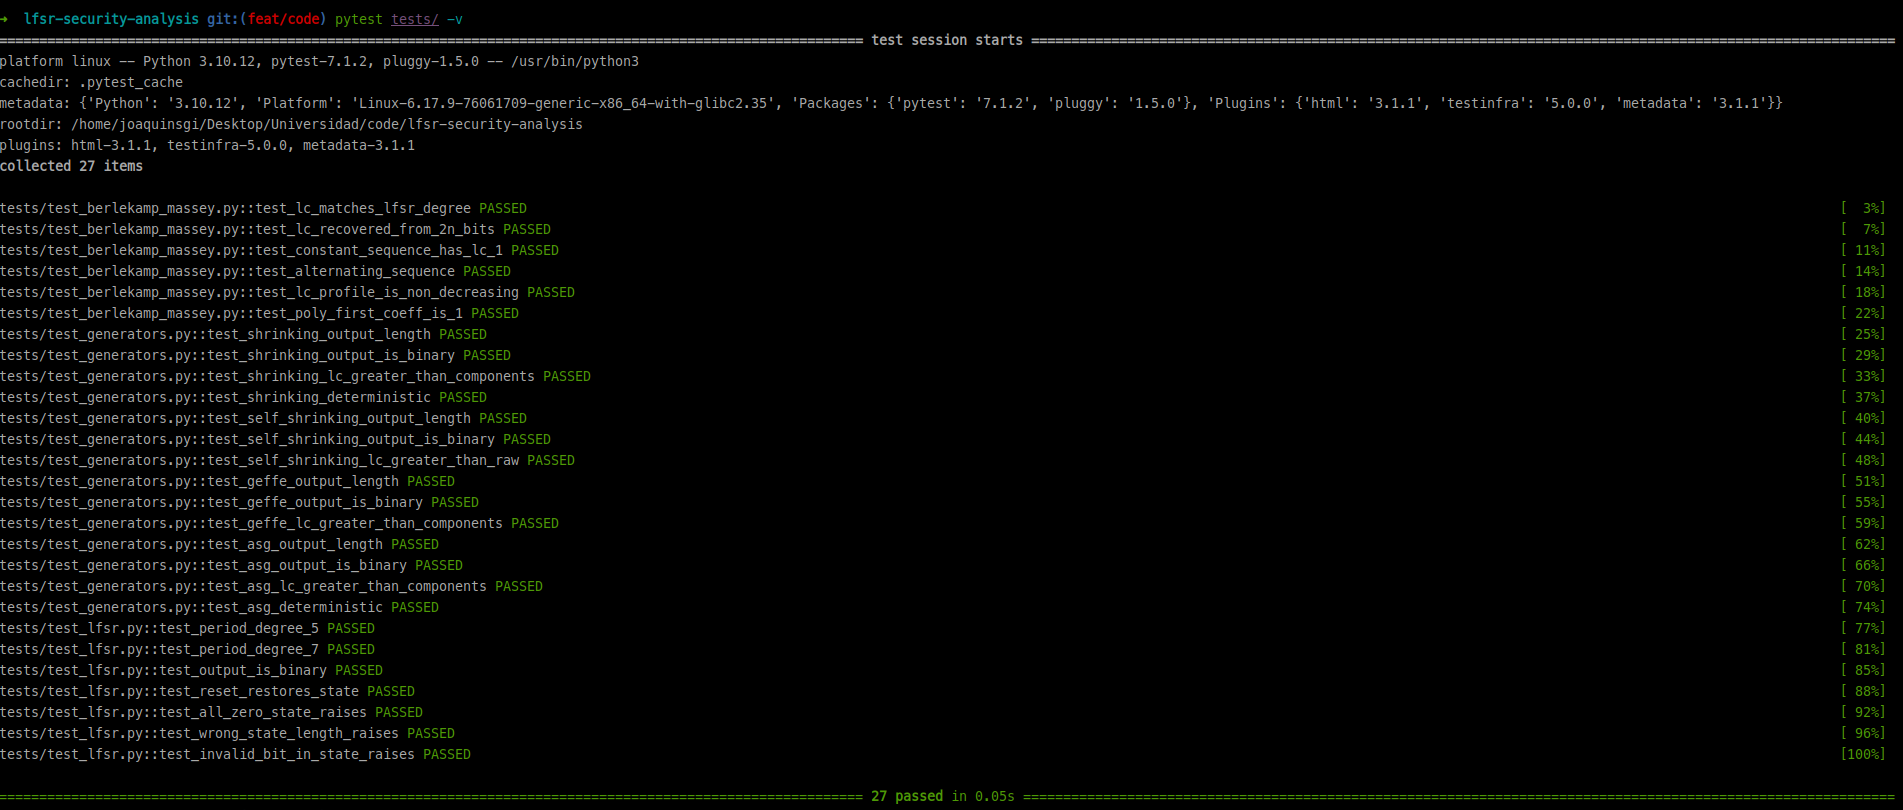
\includegraphics[width=0.9\textwidth]{images/execution_pytest.png}
\caption{Salida de \texttt{pytest tests/ -v} sobre el árbol completo.}
\label{fig:exec-pytest-appendix}
\end{figure}

Que los 27 tests pasen no garantiza que el análisis del capítulo~\ref{cap:analisis} sea correcto,
ya que los tests cubren la lógica interna pero no el experimento al completo.
Sí garantiza que cada componente aislado se comporta como se espera,
y por tanto cualquier discrepancia en los resultados experimentales no es atribuible a errores básicos de implementación.

\section{Ejecución del experimento principal}

El script \texttt{run\_experiments.py} reproduce el flujo completo del capítulo~\ref{cap:analisis}.
Genera secuencias de 500.000 bits con los cuatro generadores, calcula la complejidad lineal de los primeros 5.000 bits
con Berlekamp-Massey, aplica los ocho tests NIST a cada secuencia y serializa los resultados en \texttt{results/results.json}.

\begin{figure}[H]
\centering
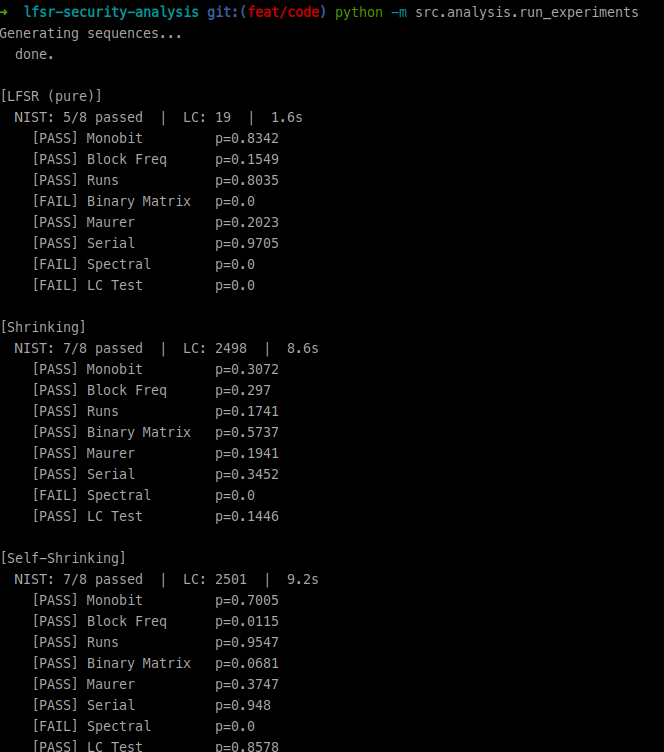
\includegraphics[width=0.9\textwidth]{images/execution_run_experiments_1.png}
\caption{Salida de \texttt{python -m src.analysis.run\_experiments} (parte 1).}
\label{fig:exec-run-experiments-app-1}
\end{figure}

\begin{figure}[H]
\centering
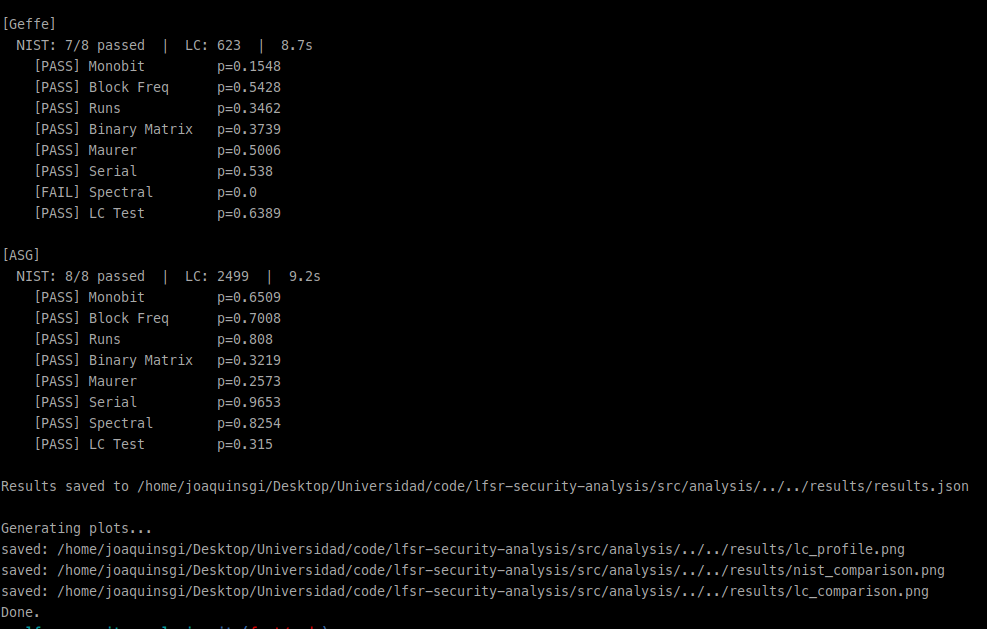
\includegraphics[width=0.9\textwidth]{images/execution_run_experiments_2.png}
\caption{Salida de \texttt{python -m src.analysis.run\_experiments} (parte 2).}
\label{fig:exec-run-experiments-app-2}
\end{figure}

Como parte de la misma ejecución, \texttt{run\_experiments.py} regenera las tres gráficas de complejidad lineal
y comparación entre generadores que aparecen en el capítulo~\ref{cap:analisis} (\texttt{results/lc\_profile.png},
\texttt{results/lc\_comparison.png} y \texttt{results/nist\_comparison.png}).

Con esto cualquier lector puede repetir el experimento completo y comparar sus resultados con los que aparecen en la memoria.
Las pequeñas variaciones en los p-valores son normales si se cambian los estados iniciales de los LFSR,
pero el comportamiento global (qué generadores pasan qué tests, qué generador obtiene complejidad lineal alta)
se mantiene estable y coincide con el análisis del capítulo~\ref{cap:analisis}.
